\documentclass[10pt]{article}
\usepackage{tikz}
\usetikzlibrary{shapes.misc}
\usepackage[margin=0cm]{geometry}
\pagestyle{empty}
\tikzstyle{every node}=[cross out, draw, red]

\begin{document}

\vspace*{\fill}
\begin{center}
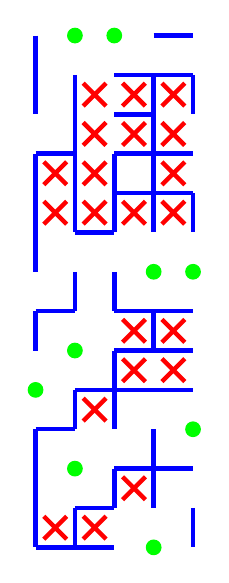
\begin{tikzpicture}[x=0.5cm, y=-0.5cm, ultra thick, blue]
% Walls
    \draw (3,0) -- (4,0);
    \draw (2,1) -- (4,1);
    \draw (2,2) -- (3,2);
    \draw (0,3) -- (1,3);
    \draw (2,3) -- (4,3);
    \draw (2,4) -- (4,4);
    \draw (1,5) -- (2,5);
    \draw (0,7) -- (1,7);
    \draw (2,7) -- (4,7);
    \draw (2,8) -- (4,8);
    \draw (1,9) -- (4,9);
    \draw (0,10) -- (1,10);
    \draw (2,11) -- (4,11);
    \draw (1,12) -- (2,12);
    \draw (0,13) -- (2,13);
    \draw (0,0) -- (0,2);
    \draw (0,3) -- (0,6);
    \draw (0,7) -- (0,8);
    \draw (0,10) -- (0,13);
    \draw (1,1) -- (1,5);
    \draw (1,6) -- (1,7);
    \draw (1,9) -- (1,10);
    \draw (1,12) -- (1,13);
    \draw (2,3) -- (2,5);
    \draw (2,6) -- (2,7);
    \draw (2,8) -- (2,10);
    \draw (2,11) -- (2,12);
    \draw (3,1) -- (3,5);
    \draw (3,7) -- (3,8);
    \draw (3,10) -- (3,12);
    \draw (4,1) -- (4,2);
    \draw (4,4) -- (4,5);
    \draw (4,12) -- (4,13);
% Pillars
    \fill[green] (1,0) circle(0.2);
    \fill[green] (2,0) circle(0.2);
    \fill[green] (3,6) circle(0.2);
    \fill[green] (4,6) circle(0.2);
    \fill[green] (1,8) circle(0.2);
    \fill[green] (0,9) circle(0.2);
    \fill[green] (4,10) circle(0.2);
    \fill[green] (1,11) circle(0.2);
    \fill[green] (3,13) circle(0.2);
% Inner points in accessible cul-de-sacs
    \node at (1.5,1.5) {};
    \node at (2.5,1.5) {};
    \node at (3.5,1.5) {};
    \node at (1.5,2.5) {};
    \node at (2.5,2.5) {};
    \node at (3.5,2.5) {};
    \node at (0.5,3.5) {};
    \node at (1.5,3.5) {};
    \node at (3.5,3.5) {};
    \node at (0.5,4.5) {};
    \node at (1.5,4.5) {};
    \node at (2.5,4.5) {};
    \node at (3.5,4.5) {};
    \node at (2.5,7.5) {};
    \node at (3.5,7.5) {};
    \node at (2.5,8.5) {};
    \node at (3.5,8.5) {};
    \node at (1.5,9.5) {};
    \node at (2.5,11.5) {};
    \node at (0.5,12.5) {};
    \node at (1.5,12.5) {};
% Entry-exit paths without intersections
\end{tikzpicture}
\end{center}
\vspace*{\fill}

\end{document}
